%% Preambel
\documentclass[conference,compsoc,final,a4paper]{IEEEtran}
\usepackage[utf8]{inputenx}

%% Bitte legen Sie hier den Titel und den Autor der Arbeit fest
\newcommand{\autoren}[0]{NACHNAME, VORNAME}
\newcommand{\dokumententitel}[0]{Vorlage für eine Seminararbeit}

% Hie muss normalerweise nichts angepasst werden
\usepackage[pdftex]{graphicx}
\graphicspath{{img/}}
\DeclareGraphicsExtensions{.pdf,.jpeg,.jpg,.png}
\usepackage[cmex10]{amsmath}
\usepackage{algorithmic}
\usepackage{array}
\usepackage{dblfloatfix}
\usepackage{url}
\usepackage[autostyle=true,german=quotes]{csquotes}
\usepackage[backend=biber]{biblatex}
\usepackage{booktabs}
\usepackage{xcolor}
\usepackage{listings}             % Source Code listings
\usepackage[printonlyused]{acronym}

% Farben definieren
\definecolor{linkblue}{RGB}{0, 0, 100}
\definecolor{linkblack}{RGB}{0, 0, 0}
\definecolor{darkgreen}{RGB}{14, 144, 102}
\definecolor{darkblue}{RGB}{0,0,168}
\definecolor{darkred}{RGB}{128,0,0}
\definecolor{comment}{RGB}{63, 127, 95}
\definecolor{javadoccomment}{RGB}{63, 95, 191}
\definecolor{keyword}{RGB}{108, 0, 67}
\definecolor{type}{RGB}{0, 0, 0}
\definecolor{method}{RGB}{0, 0, 0}
\definecolor{variable}{RGB}{0, 0, 0}
\definecolor{literal}{RGB}{31,0, 255}
\definecolor{operator}{RGB}{0, 0, 0}

\usepackage[ngerman]{betababel}
\usepackage[
	    unicode=true,
      hypertexnames=false,
      colorlinks=true,
      colorlinks=false,
      linkcolor=darkblue,
      citecolor=darkblue,
      urlcolor=darkblue,
      pdftex
   ]{hyperref}
%	 \PrerenderUnicode{ü}

% Einstellungen für Quelltexte
\lstset{
      xleftmargin=0.1cm,
      basicstyle=\scriptsize\ttfamily,
      keywordstyle=\color{keyword},
      identifierstyle=\color{variable},
      commentstyle=\color{comment},
      stringstyle=\color{literal},
      tabsize=2,
      lineskip={2pt},
      columns=flexible,
      inputencoding=utf8,
      captionpos=b,
      breakautoindent=true,
	  breakindent=2em,
	  breaklines=true,
	  prebreak=,
	  postbreak=,
      numbers=none,
      numberstyle=\tiny,
      showspaces=false,      % Keine Leerzeichensymbole
      showtabs=false,        % Keine Tabsymbole
      showstringspaces=false,% Leerzeichen in Strings
      morecomment=[s][\color{javadoccomment}]{/**}{*/},
      literate={Ö}{{\"O}}1 {Ä}{{\"A}}1 {Ü}{{\"U}}1 {ß}{{\ss}}2 {ü}{{\"u}}1 {ä}{{\"a}}1 {ö}{{\"o}}1
}

\hypersetup{
  pdftitle={\dokumententitel},
	pdfauthor={\autoren},
	pdfdisplaydoctitle=true
}

% Wo liegt Sourcecode?
\newcommand{\srcloc}{src/}

% Literatur einbinden
\addbibresource{literatur.bib}

\begin{document}

% Titel des Dokuments
\title{\dokumententitel}

% Namen der Autoren
\author{
  \IEEEauthorblockN{\autoren}
  \IEEEauthorblockA{
    Hochschule Mannheim\\
    Fakultät für Informatik\\
    Paul-Wittsack-Str. 10,
    68163 Mannheim
    }
}

% Titel erzeugen
\maketitle
\thispagestyle{plain}
\pagestyle{plain}
 % Weitere Einstellungen aus einer anderen Datei lesen

% Eigentliches Dokument beginnt hier
% ----------------------------------------------------------------------------------------------------------

% Kurze Zusammenfassung des Dokuments
\begin{abstract}
An dieser Stelle steht eine kurze Zusammenfassung des Inhaltes des Dokuments.
\end{abstract}

\tableofcontents

% Abschnitte mit \section und Unterabschnitte mit \subsection
\section{Einleitung}

Eine generelle Darstellung des Problems, der Ziele der Arbeit und deren Aufbau. Beschreibt den Hintergrund der Arbeit, das bearbeitete Problem und die Untersuchungsmethoden. Am Ende wird kurz der Aufbau der Arbeit erläutert.


\section{Kapitel mit Unterkapiteln}

\subsection{Stil der Arbeit}

Schreiben Sie die Arbeit so, dass ein fachkundiger Dritter in der Lage ist, den Text zu verstehen und die darin enthaltenen Schlüsse nachvollziehen zu können. Hierzu sollten alle nicht bekannten Fakten mit Literaturstellen belegt werden. Schreiben Sie in einer einfachen, gut verständlichen Sprache mit kurzen Sätzen. Schreiben sie durchgängig in der Gegenwartsform und im passiv (z.\,B. \enquote{\dots wird untersucht}, \enquote{\dots zeigt folgende Ergebnisse}). Nutzen Sie wenn möglich deutsche Begriffe, auf keinen Fall jedoch Mischformen wie \emph{downgeloaded} oder \emph{upgedatet}. Abkürzungen müssen in einem Abkürzungsverzeichnis aufgeführt und bei der ersten Verwendung auch ausgeschrieben werden, also z.\,B. \ac{AES} bei der ersten Verwendung, danach einfach nur \ac{AES}.


\subsection{Anmerkungen}

Zur Qualitätssicherung Ihrer Arbeit ist u.\,a. folgende Vorgehensweise hilfreich:
\begin{itemize}
\item Wenn es irgendwie möglich ist, sollten Sie die Arbeit auch Kommilitonen lesen lassen. Selbst Verwandte, Freunde und Bekannte, die nicht \emph{vom Fach} sind, finden vielleicht Fehler oder kommentieren Ihre Arbeit.
\item Um sicher zu stellen, dass Sie die hier beschriebenen Aspekte beachten, sollten Sie die Formalien z.\,B. nach jedem geschriebenen Kapitel überprüfen.
\item Lassen Sie sich von Ihrem betreuenden Professor alle Randbedingungen und Bewertungsschemata geben und fragen Sie, worauf sie achten sollen.
\end{itemize}


\section{Beispiel für eine Tabelle}

Tabellen können einfach eingebunden werden. Die Tabelle~\ref{google:numbers} zeigt, eine solche, eingebundene Tabelle.

% Tabelle
\begin{table}[!ht]
\centering
\rmfamily
\caption{Zeitbedarf für ausgewählte Aktionen, nach~\cite{Dean2012}}
\renewcommand{\arraystretch}{1.1}
\sffamily
\begin{footnotesize}
\begin{tabular}{l r}
\toprule
\textbf{Vorgang} & \textbf{Zeitbedarf} \\
\midrule
L1 cache reference                  & 0,5 ns\\
Branch mispredict                   & 5 ns\\
L2 cache reference                  & 7 ns\\
Mutex lock/unlock                   & 100 ns\\
Main memory reference               & 100 ns\\
Compress 1K bytes with Zippy        & 10.000 ns\\
Send 2K bytes over 1 Gbps network   & 20.000 ns\\
Read 1 MB sequentially from memory  & 250.000 ns\\
Round trip within same datacenter   & 500.000 ns\\
Disk seek                           & 10.000.000 ns\\
Read 1 MB sequentially from network & 10.000.000 ns\\
Read 1 MB sequentially from disk    & 30.000.000 ns\\
Send packet CA-Netherlands-CA       & 150.000.000 ns\\
\bottomrule
\end{tabular}
\end{footnotesize}
\label{google:numbers}
\end{table}


\section{Zitate und Quellenangaben}

Alle von anderen Autoren gewonnenen Erkenntnisse müssen mit Quellen belegt werden. Falls Sie wörtlich zitieren werden, so muss der Text originalgetreu in Anführungszeichen wiedergegeben werden. Wird ein Teil des Textes ausgelassen, so werden Punkte in eckigen Klammern [\,\dots] an die Stelle der Auslassung gesetzt. Zusätze innerhalb des zitierten Textes bedürfen eckiger Klammern []. Gehen Sie sparsam mit wörtlichen Zitaten um. Längere wörtliche Zitate werden i.\,a. eingerückt.

Die Zitierweise muss im gesamten Text einheitlich sein. Empfehlenswert ist beispielsweise die Harvard-Zitierweise oder die in diesem Dokument verwendete numerische Zitierweise \cite{kornmeier}.

Wichtig ist, dass das Übernehmen von fremden Textstellen ohne entsprechende Kennzeichnung der Herkunft in einer wissenschaftlichen Arbeit nicht akzeptabel ist. Plagiate werden mit der Note 5.0 bewertet.

Im Allgemeinen sind Internetquellen nicht zitierfähig, da sie oft weder dem wissenschaftlichen Anspruch genügen, noch dauerhaft zur Verfügung stehen. Falls trotzdem eine Quelle aus dem Internet zitiert werden muss, z.\,B. weil weder Bücher noch Zeitschriften die Information liefern, so muss ein Ausdruck der Webseite mit Datum und Internetadresse im Anhang angehängt oder als PDF auf CD beigelegt werden.

\section{Abbildungen}

Abbildungen sind oft sehr hilfreich, um Zusammenhänge zu verdeutlichen. Soweit möglich, sollten die Abbildungen als Vektorgrafiken eingebunden werden. Die in der Abbildung enthaltenen Schriftarten sollten nach Möglichkeit die gleichen sein, wie im restlichen Dokument. Alle Beschriftungen innerhalb der Grafik sollten gut lesbar sein.
Graphen können farbig sein, wenn es der Lesbarkeit dient. Es sollte jedoch darauf geachtet werden, dass auch eine schwarz\-weiß-Kopie noch alle nötigen Informationen enthält (d.h. Liniendiagramme mit verschiedenen Linienarten z.\,B. Strichpunkt).
Falls eine Abbildung nur in Form einer Bitmap realisiert werden kann (e,\.B. Screenshot), sollte die Auflösung mindestens 600 dpi betragen und die Qualität nicht durch Komprimierung (z.\,B. jpg) verschlechtert werden. Unkomprimierte oder verlustfrei komprimierte Bildformate wie \emph{png} oder \emph{bmp} sind zu bevorzugen. Nur für echte Fotos ist \emph{jpg} geeignet.

% Grafik in einer Spalte
\begin{figure}[!ht]
\centering
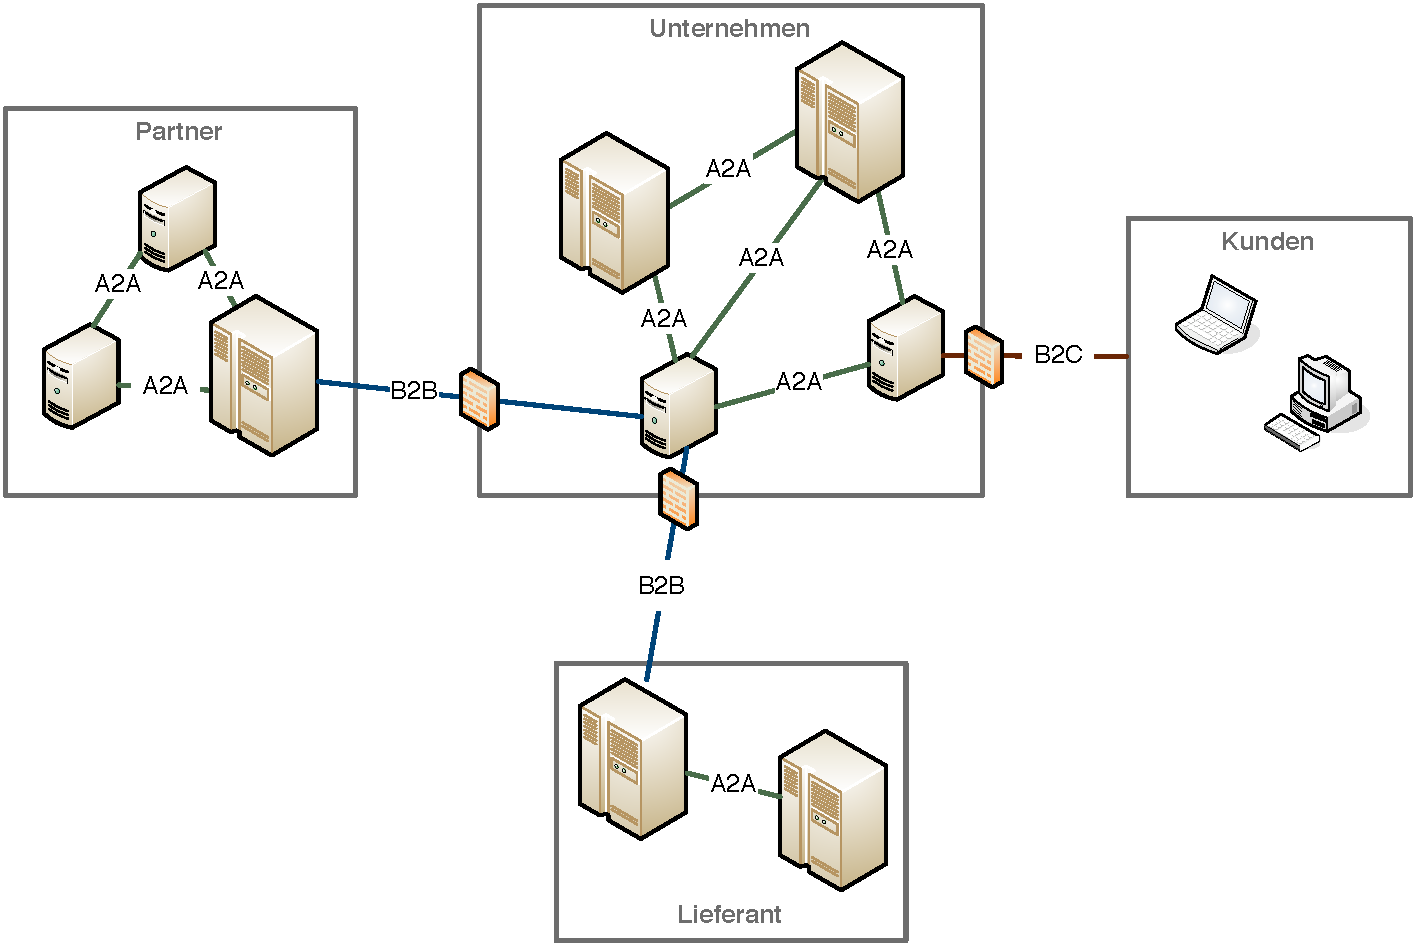
\includegraphics[width=8.5cm]{bsp1}
\caption{Beispielgrafik~\cite{Dean2012}}
\label{fig_sim}
\end{figure}

Jede Abbildung (vgl. Abbildung~\ref{fig_sim} auf Seite~\pageref{fig_sim}) und Tabelle (z.\,B. Tabelle~\ref{google:numbers} auf Seite~\pageref{google:numbers}) sollte im Fließtext referenziert und behandelt werden. Die Beschriftung unter den Abbildungen sollte die Abbildung vollständig und verständlich beschreiben, auch ohne dass man den restlichen Text gelesen hat. Gleiches gilt für die Beschriftungen von Tabellen, die über die Tabellen gesetzt werden.

\section{Formelsatz}

Eine Formel gefällig? Mitten im Text $a_2 = \sqrt{x^3}$ oder als eigener Absatz (siehe Formel~\ref{Formel}):

\begin{equation}
\begin{bmatrix}
   1 &  4 &  2 \\
   4 &  0 & -3
\end{bmatrix}
        \cdot
\begin{bmatrix}
   1 &  1 &  0 \\
  -2 &  3 &  5 \\
   0 &  1 &  4
\end{bmatrix}
       {=}
\begin{bmatrix}
  -7 &  15 &  28 \\
   4 &   1 & -12
\end{bmatrix}
\label{Formel}
\end{equation}
\\

\section{Sourcecode}

Man kann mit Latex auch einfach Sourcecode in den Text aufnehmen.

\subsection{Aus einer Datei}

\lstinputlisting[firstline=2,language=Java,caption={Das Interface Crypter}]{\srcloc/Crypter.java}


\subsection{Inline}

\begin{lstlisting}[language=Java,caption=Methode checkKey()]
/**
 * Testet den Schlüssel auf Korrektheit: Er muss
 * mindestens die Länge 1 haben und darf nur
 * Zeichen von A-Z enthalten.
 *
 * @param key zu testender Schlüssel
 * @throws CrypterException wenn der Schlüssel nicht
 * OK ist.
 */
protected void checkKey(Key key) throws CrypterException {

    // Passt die Länge?
    if (key.getKey().length == 0) {
        throw new CrypterException("Der Schlüssel muss mindestens " +
                "ein Zeichen lang sein");
    }

    checkCharacters(key.getKey(), ALPHABET);
}
\end{lstlisting}


%% --------------------------------------------------------------------

\section*{Abkürzungen}
\addcontentsline{toc}{section}{Abkürzungen}

\begin{acronym}
\acro{A2A}{Application-to-Application}
\acro{ACL}{Acess Control List}
\acro{AES}{Advanced Encryption Standard}
\end{acronym}

% Literaturverzeichnis
\addcontentsline{toc}{section}{Literatur}
\printbibliography

\end{document}
